
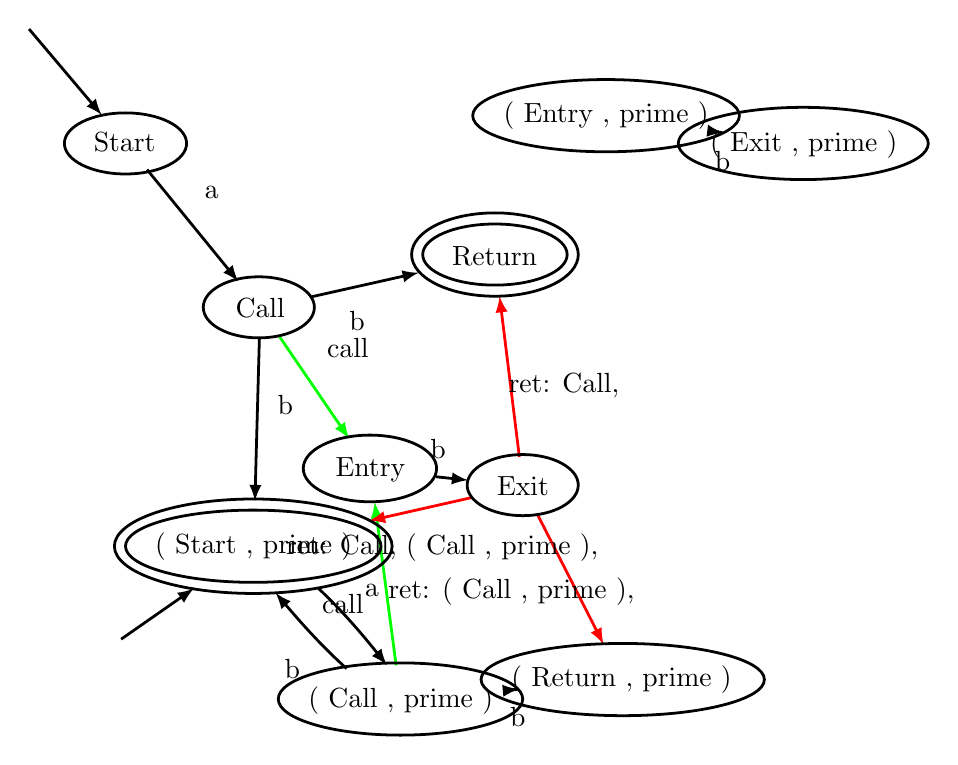
\begin{tikzpicture}[>=latex,line join=bevel,]
  \pgfsetlinewidth{1bp}
%%
\pgfsetcolor{black}
  % Edge: ( Call , prime ) -> Entry
  \pgfsetcolor{green}
  \draw [->] (173.43bp,28.126bp) .. controls (171.74bp,40.97bp) and (169.08bp,61.144bp)  .. (165.7bp,86.861bp);
  \definecolor{strokecol}{rgb}{0.0,0.0,0.0};
  \pgfsetstrokecolor{strokecol}
  \draw (154.24bp,50.366bp) node {call};
  % Edge: Exit -> Return
  \pgfsetcolor{red}
  \draw [->] (217.79bp,103.18bp) .. controls (216.32bp,115.07bp) and (213.88bp,134.87bp)  .. (210.66bp,160.99bp);
  \definecolor{strokecol}{rgb}{0.0,0.0,0.0};
  \pgfsetstrokecolor{strokecol}
  \draw (233.86bp,128.97bp) node {ret: Call, };
  % Edge: Call -> Entry
  \pgfsetcolor{green}
  \draw [->] (131.4bp,146.52bp) .. controls (136.72bp,138.73bp) and (144.23bp,127.72bp)  .. (156.52bp,109.71bp);
  \definecolor{strokecol}{rgb}{0.0,0.0,0.0};
  \pgfsetstrokecolor{strokecol}
  \draw (156.06bp,142.37bp) node {call};
  % Edge: ( Entry , prime ) -> ( Exit , prime )
  \draw [->] (290.83bp,219.91bp) .. controls (290.9bp,219.9bp) and (290.96bp,219.89bp)  .. (291.2bp,219.86bp);
  \draw (290.93bp,209.9bp) node {b};
  % Edge: Exit -> ( Return , prime )
  \pgfsetcolor{red}
  \draw [->] (224.32bp,82.402bp) .. controls (229.36bp,72.509bp) and (237.14bp,57.241bp)  .. (248.1bp,35.704bp);
  \definecolor{strokecol}{rgb}{0.0,0.0,0.0};
  \pgfsetstrokecolor{strokecol}
  \draw (214.93bp,54.533bp) node {ret: ( Call , prime ), };
  % Edge: Start -> Call
  \draw [->] (83.755bp,206.6bp) .. controls (90.932bp,197.8bp) and (101.6bp,184.72bp)  .. (116.59bp,166.34bp);
  \draw (106.99bp,198.37bp) node {a};
  % Edge: ( Call , prime ) -> ( Return , prime )
  \draw [->] (217.16bp,19.489bp) .. controls (217.23bp,19.496bp) and (217.31bp,19.504bp)  .. (217.6bp,19.532bp);
  \draw (217.27bp,9.5bp) node {b};
  % Edge: Exit -> ( Start , prime )
  \pgfsetcolor{red}
  \draw [->] (200.4bp,88.458bp) .. controls (192.64bp,86.706bp) and (183.22bp,84.577bp)  .. (163.66bp,80.16bp);
  \definecolor{strokecol}{rgb}{0.0,0.0,0.0};
  \pgfsetstrokecolor{strokecol}
  \draw (190.02bp,70.436bp) node {ret: Call, ( Call , prime ), };
  % Edge: Start__precursor__ -> Start
  \draw [->] (41.286bp,257.18bp) .. controls (47.309bp,250.06bp) and (54.459bp,241.6bp)  .. (67.423bp,226.27bp);
  % Edge: Entry -> Exit
  \draw [->] (187.77bp,96.004bp) .. controls (188.25bp,95.953bp) and (188.74bp,95.902bp)  .. (199.29bp,94.782bp);
  \draw (188.5bp,105.93bp) node {b};
  % Edge: Call -> ( Start , prime )
  \draw [->] (124.21bp,146.12bp) .. controls (123.88bp,134.07bp) and (123.32bp,113.88bp)  .. (122.6bp,87.286bp);
  \draw (133.54bp,121.77bp) node {b};
  % Edge: Call -> Return
  \draw [->] (143.22bp,160.85bp) .. controls (151.58bp,162.73bp) and (161.74bp,165.01bp)  .. (181.54bp,169.45bp);
  \draw (159.38bp,152.03bp) node {b};
  % Edge: ( Call , prime ) -> ( Start , prime )
  \draw [->] (155.62bp,26.951bp) .. controls (149.26bp,32.647bp) and (142.35bp,39.689bp)  .. (130.03bp,54.223bp);
  \draw (136.02bp,26.712bp) node {b};
  % Edge: ( Start , prime ) -> ( Call , prime )
  \draw [->] (145.34bp,55.932bp) .. controls (151.78bp,49.847bp) and (158.47bp,42.747bp)  .. (170.05bp,28.27bp);
  \draw (164.63bp,55.057bp) node {a};
  % Edge: ( Start , prime )__precursor__ -> ( Start , prime )
  \draw [->] (74.436bp,37.537bp) .. controls (79.915bp,41.355bp) and (86.038bp,45.622bp)  .. (100.6bp,55.769bp);
  % Node: Return
\begin{scope}
  \definecolor{strokecol}{rgb}{0.0,0.0,0.0};
  \pgfsetstrokecolor{strokecol}
  \draw (209bp,176bp) ellipse (26bp and 11bp);
  \draw (209bp,176bp) ellipse (30bp and 15bp);
  \draw (208.86bp,175.58bp) node {Return};
\end{scope}
  % Node: ( Start , prime )
\begin{scope}
  \definecolor{strokecol}{rgb}{0.0,0.0,0.0};
  \pgfsetstrokecolor{strokecol}
  \draw (122bp,71bp) ellipse (46bp and 13bp);
  \draw (122bp,71bp) ellipse (50bp and 17bp);
  \draw (122.14bp,70.781bp) node {( Start , prime )};
\end{scope}
  % Node: Exit
\begin{scope}
  \definecolor{strokecol}{rgb}{0.0,0.0,0.0};
  \pgfsetstrokecolor{strokecol}
  \draw (219bp,93bp) ellipse (20bp and 11bp);
  \draw (219.09bp,92.681bp) node {Exit};
\end{scope}
  % Node: ( Call , prime )
\begin{scope}
  \definecolor{strokecol}{rgb}{0.0,0.0,0.0};
  \pgfsetstrokecolor{strokecol}
  \draw (175bp,16bp) ellipse (44bp and 13bp);
  \draw (175.09bp,15.522bp) node {( Call , prime )};
\end{scope}
  % Node: ( Exit , prime )
\begin{scope}
  \definecolor{strokecol}{rgb}{0.0,0.0,0.0};
  \pgfsetstrokecolor{strokecol}
  \draw (320bp,216bp) ellipse (45bp and 13bp);
  \draw (320.21bp,215.52bp) node {( Exit , prime )};
\end{scope}
  % Node: ( Entry , prime )
\begin{scope}
  \definecolor{strokecol}{rgb}{0.0,0.0,0.0};
  \pgfsetstrokecolor{strokecol}
  \draw (249bp,226bp) ellipse (48bp and 13bp);
  \draw (249bp,226.16bp) node {( Entry , prime )};
\end{scope}
  % Node: Start
\begin{scope}
  \definecolor{strokecol}{rgb}{0.0,0.0,0.0};
  \pgfsetstrokecolor{strokecol}
  \draw (76bp,216bp) ellipse (22bp and 11bp);
  \draw (75.697bp,216.48bp) node {Start};
\end{scope}
  % Node: Call
\begin{scope}
  \definecolor{strokecol}{rgb}{0.0,0.0,0.0};
  \pgfsetstrokecolor{strokecol}
  \draw (124bp,157bp) ellipse (20bp and 11bp);
  \draw (124.49bp,156.65bp) node {Call};
\end{scope}
  % Node: Entry
\begin{scope}
  \definecolor{strokecol}{rgb}{0.0,0.0,0.0};
  \pgfsetstrokecolor{strokecol}
  \draw (164bp,99bp) ellipse (24bp and 12bp);
  \draw (164.16bp,98.509bp) node {Entry};
\end{scope}
  % Node: ( Return , prime )
\begin{scope}
  \definecolor{strokecol}{rgb}{0.0,0.0,0.0};
  \pgfsetstrokecolor{strokecol}
  \draw (255bp,23bp) ellipse (51bp and 13bp);
  \draw (254.57bp,23.018bp) node {( Return , prime )};
\end{scope}
%
\end{tikzpicture}
